\chapter{Controllo della concorrenza}
La maggior parte della teoria del controllo della concorrenza nelle basi di dati è stata sviluppata per sistemi di calcolo con una sola CPU. In tali sistemi i programmi sono eseguiti concorrentemente in modo interleaved (interfogliato): la CPU può eseguire un solo programma alla volta, tuttavia il sistema operativo permette di eseguire alcune istruzioni di un programma, sospendere quel programma, eseguire istruzioni di un altro programma e quindi ritornare ad eseguire istruzioni del primo.

\section{Introduzione alla concorrenza}
In un sistema di gestione di basi di dati multiutente la principale risorsa a cui i vari programmi accedono concorrentemente è la base di dati. L'esecuzione di una parte di un programma che rappresenta un'unità logica di accesso o modifica del contenuto della base di dati è detta transazione. Nei sistemi in cui vengono effettuate da più
utenti sia operazioni di lettura che di scrittura l'esecuzione concorrente di più transazioni può provocare problemi se non viene controllata in qualche modo. Perché le transazioni operino in modo corretto sui dati è necessario che i meccanismi che le implementano soddisfino queste quattro proprietà: 
\begin{itemize}
    \item \textit{Atomicità}: la transazione è indivisibile nella sua esecuzione, infatti la sua esecuzione deve essere o totale o nulla e non sono ammesse esecuzioni parziali;
    \item \textit{Consistenza}: quando inizia una transazione il database si trova in uno stato consistente e quando la transazione termina il database deve essere in un altro stato consistente, ovvero non deve violare eventuali vincoli di integrità;
    \item \textit{Isolamento}: ogni transazione deve essere eseguita in modo isolato e indipendente dalle altre transazioni, l'eventuale fallimento di una transazione non deve interferire con le altre transazioni in esecuzione;
    \item \textit{Durabilità}: si riferisce al fatto che una volta che una transazione abbia richiesto un commit work, i cambiamenti apportati non dovranno essere più persi. Per evitare che nel lasso di tempo fra il momento in cui la base di dati si impegna a scrivere le modifiche e quello in cui li scrive effettivamente si verifichino perdite di dati dovuti a malfunzionamenti, vengono tenuti dei registri di log dove sono annotate tutte le operazioni sul DB.
\end{itemize}

Prima di esaminare alcuni dei problemi che possono sorgere quando l'esecuzione concorrente di più transazioni non è controllata, introduciamo il concetto di schedule (piano di esecuzione) di un insieme di transazioni. Dato un insieme T di transazioni uno \textit{schedule} S di T è un ordinamento delle operazioni nelle transazioni in T tale che per ogni transazione T in T se o1 e o2 sono due operazioni in T tali che o1 precede o2 in T allora o1 precede o2 in S (in altre parole uno schedule deve conservare l'ordine che le operazioni hanno all'interno delle singole transazioni). Qualsiasi schedule ottenuto permutando le transazioni in T è detto \textit{seriale}.

Consideriamo le seguenti transazioni e i seguenti schemi di $T_1, T_2$:
\begin{center}
    \begin{tabular}{|c|c|}
         \hline$T_1$&$T_2$\\\hline
         read(X)& \\
         X:=X-N& \\
         &read(X) \\
         &X:=X+M \\
         write(X)& \\
         read(Y)& \\
         &write(X) \\
         Y:=Y+N& \\
         write(Y)& \\\hline
    \end{tabular}
    \begin{tabular}{|c|c|}
         \hline$T_1$&$T_2$\\\hline
         read(X)& \\
         X:=X-N& \\
         write(X)& \\
         &read(X) \\
         &X:=X+M \\
         &write(X) \\
         read(Y)& \\
         $T_1$ fallisce& \\
         &write(X) \\\hline
    \end{tabular}
    \begin{tabular}{|c|c|}
         \hline$T_1$&$T_3$\\\hline
         &somma:=0 \\
         read(X)& \\
         X:=X-N& \\
         write(X)& \\
         &read(X) \\
         &somma:=somma+X \\
         &read(Y) \\
         &somma:=somma+Y \\
         read(Y)& \\
         Y:=Y+N& \\
         write(Y)& \\\hline
    \end{tabular}
\end{center}

Nel primo caso l'aggiornamento di X prodotto da $T_1$ viene perso in quanto $T_2$ legge il valore di X prima che l'aggiornamento prodotto da $T_1$ sia stato reso permanente. Nel secondo caso $T_2$ legge e aggiorna il valore di X dopo che l'aggiornamento prodotto da $T_1$ è stato reso permanente, ma prima che venga ripristinato il vecchio valore di X in conseguenza del fallimento di $T_1$. Consideriamo ora la transazione $T_3$ che somma i valori di X e di Y. Il seguente schedule di fa sì che la somma prodotta da $T_3$ sia la somma del valore di X dopo che X è stato aggiornato da $T_1$ e del valore di Y prima che sia stato aggiornato da $T_1$.

In tutti e tre i casi visti siamo portati a considerare gli schedule non corretti in quanto i valori prodotti non sono quelli che si avrebbero se le due transazioni fossero eseguite nel modo “naturale” cioè sequenzialmente. In generale possiamo osservare che l'esecuzione naturale e, quindi, intuitivamente corretta di un insieme di transazioni è quella sequenziale; la possibilità di eseguire concorrentemente un insieme di transazioni, come si è detto, è introdotta nei sistemi per motivi di efficienza. Pertanto tutti gli schedule seriali sono corretti e uno schedule non seriale è corretto se è serializzabile, cioè se è “equivalente” ad uno schedule seriale. Sorge quindi la necessità di definire un concetto di equivalenza di schedule.

Due schedule sono \textit{equivalenti} se (per ogni dato modificato) producono valori uguali, dove due valori sono uguali solo se sono prodotti dalla stessa sequenza di operazioni. Ad esempio i seguenti due schedule non sono considerati equivalenti:
\begin{center}
    \begin{tabular}{|c|c|}
        \hline $T_1$&$T_2$ \\\hline
        read(X)& \\
        X:=X+N& \\
        write(X)& \\
        &read(X) \\
        &X:=X-M \\
        &write(X) \\\hline
    \end{tabular}
    \begin{tabular}{|c|c|}
        \hline$T_1$&$T_2$ \\\hline
        &read(X) \\
        &X:=X-M \\
        &write(X) \\
        read(X)& \\
        X:=X+N& \\
        write(X)& \\\hline
    \end{tabular}
\end{center}

Oltre alla definizione di equivalenza, un altro elemento che ha influenza sulla complessità del problema di decidere se uno schedule è \textit{serializzabile} (cioè se è equivalente ad uno schedule seriale). Nella pratica è difficile testare la serializzabilità di uno schedule. Infatti l'ordine di esecuzione delle operazioni delle diverse transazioni è determinato in base a diversi fattori: il carico del sistema, l'ordine temporale in cui le transazioni vengono sottomesse al sistema e le loro priorità. Pertanto è praticamente impossibile determinare in anticipo come le operazioni saranno interleaved, cioè in quale ordine verranno eseguite; d'altra parte, se prima si eseguono le operazioni e poi si testa la serializzabilità dello schedule, i suoi effetti devono essere annullati se lo schedule risulta non serializzabile. Quindi l'approccio seguito nei sistemi è quello di determinare metodi che garantiscano la serializzabilità di uno schedule eliminando così la necessità di dover testare ogni volta la serializzabilità di uno schedule. Uno di tali metodi consiste nell'imporre dei protocolli, cioè delle regole, alle transazioni in modo da garantire la serializzabilità di ogni schedule. Questi protocolli usano tecniche di locking (cioè di controllo dell'accesso ai dati) per prevenire l'accesso concorrente ai dati. Altri metodi di controllo usano i timestamp delle transazioni, cioè degli identificatori delle transazioni che vengono generati dal sistema e in base ai quali le operazioni delle transazioni possono essere ordinate in modo da assicurare la serializzabilità.

\section{Item}
Tutte le tecniche per la gestione della concorrenza richiedono che la base di dati sia partizionata in item, cioè in unità a cui l'accesso è controllato. Le dimensioni degli item devono essere definite in base all'uso che viene fatto della base di dati in modo tale che in media una transazione acceda a pochi item. Le dimensioni degli item usate da un sistema sono dette la sua granularità. Una granularità grande permette una gestione efficiente della concorrenza; una piccola granularità può invece sovraccaricare il sistema, ma consente l'esecuzione concorrente di molte transazioni.

\section{Locking}
Un lock viene
richiesto da una transazione mediante un'operazione di locking e viene rilasciato mediante un'operazione di unlocking; fra l'esecuzione di un'operazione di locking su un certo item X e l'esecuzione di un'operazione di unlocking su X diciamo che la transazione mantiene un lock su X. Il locking agisce come primitiva di sincronizzazione, cioè se una transazione richiede un lock su un item su cui un'altra transazione mantiene un lock, la transazione non può procedere finchè il lock non viene rilasciato dalla prima transazione. Uno schedule è detto legale se una transazione effettua un locking ogni volta che deve leggere o scrivere un item e ciascuna transazione rilascia ogni lock che ha ottenuto.

\subsection{Lock binario}
Un lock binario può assumere solo due valori \textit{locked} e \textit{unlocked}. Le transazioni fanno uso di due operazioni lock(X) e unlock(X); la prima serve per richiedere l'accesso all'item X, la seconda per rilasciare l'item X consentendone l'accesso ad altre transazioni.

Consideriamo di nuovo le due transazioni dell'esempio precedente e vediamo come l'uso dei lock può prevenire il problema dell'”aggiornamento perso”:
\begin{center}
    \begin{tabular}{|c|c|}
        \hline $T_1$&$T_2$ \\\hline
        lock(X)& \\
        read(X)& \\
        X:=X-N& \\
        write(X)& \\
        unlock(X)& \\
        & lock(X)\\
        & read(X)\\
        & X:=X+M\\
        & write(X)\\
        & unlock(X)\\
        lock(Y)& \\
        read(Y)& \\
        Y:=Y+N& \\
        write(Y)& \\
        unlock(Y)& \\\hline
    \end{tabular}
\end{center}

Il più semplice modello per le transazioni è quello che considera una transazione come una sequenza di operazioni di lock e unlock. Si assume che ogni operazione di lock su un item X implica la lettura di X e ogni operazione di unlock di un item X implica la scrittura di X. Il nuovo valore dell'item viene calcolato da una funzione che è associata in modo univoco ad ogni coppia lock-unlock ed ha per argomenti tutti gli item letti (locked) dalla transazione prima dell'operazione di unlock.

Due schedule sono equivalenti se le formule che danno i valori finali per ciascun item sono le stesse per i due schedule. Consideriamo ora le due transazioni e i seguenti schedule di $T_1 ,T_2$:
\begin{center}
    \begin{tabular}{|c|}
        \hline $T_1$\\\hline
        lock(X)\\
        unlock(X) $f_1$(X)\\
        lock(Y)\\
        unlock(Y)\\
        $f_2$(X,Y)\\\hline
    \end{tabular}
    \begin{tabular}{|c|}
        \hline $T_2$\\\hline
        lock(Y)\\
        unlock(Y) $f_3$(Y)\\
        lock(X)\\
        unlock(X)\\
        $f_4$(X,Y)\\\hline
    \end{tabular}\hspace{1cm}
    \begin{tabular}{|c|c|}
        \hline $T_1$&$T_2$ \\\hline
        lock(X) & \\
        unlock(X) & \\
        & lock(Y)\\
        & unlock(Y)\\
        lock(Y) & \\
        unlock(Y) & \\
        & lock(X)\\
        & unlock(X)\\\hline
    \end{tabular}
\end{center}
Se indichiamo con $X_0$ e $Y_0$ i valori iniziali di X e Y, abbiamo che il valore finale per X prodotto da S è dato dalla formula $f_4 (f_1 (X_0 ), Y_0)$. D'altra parte il valore finale per X prodotto dallo schedule seriale $T_1 ,T_2$ è dato dalla formula $f_4 (f_1 (X_0 ), f_2 (X_0,Y_0))$, mentre il valore finale per X prodotto dallo schedule seriale $T_2 ,T_1$ è dato dalla formula $f_1 (f_4 (X_0 , Y_0 ))$; pertanto S non è serializzabile in quanto non è equivalente a nessuno schedule seriale di $T1 ,T_2$.

Consideriamo ora le due transazioni e i seguenti schedule di $T_1 ,T_2$:
\begin{center}
    \begin{tabular}{|c|}
        \hline $T_1$\\\hline
        lock(X)\\
        unlock(X) $f_1$(X)\\
        lock(Y)\\
        unlock(X)\\
        $f_2$(X,Y)\\\hline
    \end{tabular}
    \begin{tabular}{|c|}
        \hline $T_2$\\\hline
        lock(X)\\
        unlock(X) $f_3$(X)\\
        lock(Y)\\
        unlock(Y)\\
        $f_4$(X,Y)\\\hline
    \end{tabular}\hspace{1cm}
    \begin{tabular}{|c|c|}
        \hline $T_1$&$T_2$ \\\hline
        lock(X) & \\
        unlock(X) & \\
        & lock(X)\\
        & unlock(X)\\
        lock(Y) & \\
        unlock(Y) & \\
        & lock(Y)\\
        & unlock(Y)\\\hline
    \end{tabular}
\end{center}
Se indichiamo con $X_0$ e $Y_0$ i valori iniziali di X e Y, abbiamo che il valore finale per X e Y prodotti da S sono dati rispettivamente dalle formule $f_3 (f_1 (X_0 ))$ e $f_4 (f_1 (X_0 ), f_2 (X_0,Y_0))$. Poiché tali formule coincidono con quelle prodotte dallo schedule seriale $T_1 ,T_2$ lo schedule S è serializzabile.

La serializzabilità di uno schedule in questo semplice modello, può essere testata mediante un semplice algoritmo su grafi diretti. L'idea su cui si basa tale algoritmo è la seguente. Dato uno schedule, per ogni item si esamina l'ordine in cui le varie transazioni fanno un lock su quell'item; se lo schedule è serializzabile questo ordine deve essere consistente con quello di uno schedule seriale; pertanto se l'ordine imposto sulle transazioni da un certo item è diverso da quello imposto da un altro item, lo schedule non è serializzabile.

\begin{Algoritmo}{Serializzabilità di uno schedule}{}
    Dato uno schedule S:
    \begin{itemize}
        \item Crea un grafo diretto G (grafo di serializzazione) i cui nodi corrispondono alle transazioni; in tale grafo c'è un arco diretto da $T_i$ a $T_j$ (con eichetta X) se in S $T_i$ esegue un unlock(X) e $Tj$ esegue il successivo lock(X);
        \item Se G ha un ciclo allora S non è serializzabile; altrimenti applicando a G l'ordinamento topologico (eliminando ricorsivamente i nodi del grafo che non hanno archi entranti) si ottiene uno schedule seriale S' equivalente ad S.
    \end{itemize}
\end{Algoritmo}

\begin{Thm}{Correttezza dell'Algoritmo del grafo di serializzazione}{}\label{thm:correttezza-grafo-serializzazione}
    Uno schedule S è serializzabile se e solo se il suo grafo di serializzazione è aciclico.
\end{Thm}

Diciamo che una transazione obbedisce al protocollo di \textit{locking a due fasi}, o più semplicemente che è a due fasi, se prima effettua tutte le operazioni di lock (fase di locking) e poi tutte le operazioni di unlock (fase di unlocking).

\begin{Thm}{Locking a due fasi è serializzabile}{}
    Sia T un insieme di transazioni. Se ogni transazione in T è a due fasi allora ogni schedule di T è serializzabile.
    \begin{demonstration}
        Sia S uno schedule di T. Supponiamo, per assurdo, che S non sia serializzabile. Per il Teorema \ref{thm:correttezza-grafo-serializzazione}, il grafo di serializzazione G di S contiene un ciclo $T_1, T_2 ,..., T_k$ , $T_1$; ciò significa che $T_{i+1}$, $i=1,... k-1$, effettua un'operazione di lock, su un item su cui $T_i$ ha effettuato un'operazione di unlock e che $T_1$ effettua un'operazione di lock, su un item su cui $T_k$ ha effettuato un'operazione di unlock. Pertanto in S $T_1$ effettua un'operazione di lock dopo aver effettuato un'operazione di unlock e quindi $T_1$ non è a due fasi (contraddizione).
    \end{demonstration}
\end{Thm}

Mostreremo ora che se una transazione $T_1$ non è a due fasi, esiste sempre una transazione $T_2$ tale che esiste uno schedule di $T_1, T2$ che non è serializzabile. Infatti, se $T_1$ non è a due fasi effettua un'operazione di lock dopo aver effettuato un'operazione di unlock:
\begin{center}
    \begin{tabular}{|c|}
        \hline $T_1$\\\hline
        ...\\
        unlock(X)\\
        ...\\
        lock(Y)\\
        ...\\\hline
    \end{tabular}
    \begin{tabular}{|c|}
        \hline $T_2$\\\hline
        lock(X)\\
        lock(Y)\\
        unlock(X)\\
        unlock(Y)\\\hline
    \end{tabular}\hspace{1cm}
    \begin{tabular}{|c|c|}
        \hline $T_1$&$T_2$\\\hline
        ...& \\
        unlock(X)& \\
        ...& \\
        & lock(X)\\
        & lock(Y)\\
        & unlock(X)\\
        & unlock(Y)\\
        ...& \\
        lock(Y)& \\
        ...& \\\hline
    \end{tabular}\hspace{1cm}
    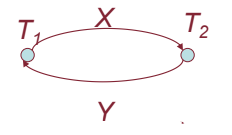
\includegraphics[width=0.2\linewidth]{images/esempio-lock-due-valori.PNG}
\end{center}

Naturalmente possono esistere schedule di transazioni che non sono a due fasi che sono serializzabili. Tuttavia poiché è normale non conoscere l'insieme di transazioni con cui una transazione può essere eseguita concorrentemente siamo costretti a richiedere che tutte le transazioni siano a due fasi perché sia garantita la serializzabilità di ogni schedule.

\section{Deadlock e livelock}
In un sistema che utilizza i lock per il controllo della concorrenza si possono verificare delle situazioni anomale note con il nome di deadlock e livelock.

Un livelock si verifica quando una transazione aspetta indefinitamente che gli venga garantito un lock su un certo item. 

Un deadlock si verifica quando ogni transazione in un insieme T è in attesa di ottenere un lock su un item sul quale qualche altra transazione in T mantiene un lock. 

Il primo problema può essere risolto con una strategia first came-first served; in altre parole il sistema mantiene memoria delle successive richieste di lock in modo che, quando un item X viene rilasciato, viene garantito un lock su X alla transazione che per prima ha richiesto un lock su X. Un'altra possibile strategia può essere quella di eseguire le transazioni in base alle loro priorità e di aumentare la priorità di una transazione all'aumentare del tempo in cui rimane in attesa in modo che possa ad un certo punto assumere la priorità più alta ed essere eseguita.

Per risolvere il secondo problema possono essere seguiti due approcci. Un approccio è preventivo in quanto cerca di evitare il verificarsi di situazioni di stallo adottando opportuni protocolli; l'altro invece si preoccupa di risolvere le situazioni di stallo quando si verificano. Il sussistere di una situazione di stallo può essere rilevato mantenendo un grafo di attesa, cioè un grafo i cui nodi sono le transazioni e in cui c'è un arco $T_1\to T_2$ se la transazione $T_1$ è in attesa di ottenere un lock su un item sul quale $T_2$ mantiene un lock; se in tale grafo c'è un ciclo si sta verificando una situazione di stallo che coinvolge le transazioni nel ciclo; per risolverla occorre che almeno una transazione nel ciclo sia rolled-back (cioè la transazione viene abortita, i suoi effetti sulla base di dati vengono annullati ripristinando i valori dei dati precedenti l'inizio della sua esecuzione e, infine, tutti i lock mantenuti dalla transazione vengono rilasciati) e quindi venga fatta ripartire.

\section{Locking a due fasi stretto}
Oltre al verificarsi di un deadlock, ci sono altri motivi per cui una transazione deve essere abortita, ad esempio: perché ha cercato di effettuare un accesso non autorizzato oppure perché ha cercato di eseguire una divisione per 0. Il punto in cui una transazione non può più essere abortita per uno dei suddetti motivi, cioè il punto in cui ha ottenuto tutti i lock che gli sono necessari e ha effettuato tutti i calcoli nell'area di lavoro, viene detto punto di commit della transazione; una transazione che ha raggiunto il suo punto di commit viene detta committed altrimenti viene detta attiva. Quando una transazione raggiunge il suo punto di commit effettua un'operazione di commit (nei sistemi reali tale operazione prevede lo svolgimento di diverse azioni, ma per i nostri scopi serve solo a marcare il punto di commit della transazione). I dati scritti da una transazione sulla base di dati prima che abbia raggiunto il punto di commit vengono detti dati sporchi. Il fatto che un dato sporco possa essere letto da qualche altra  transazione può causare un effetto di roll-back a cascata. Consideriamo il seguente schedule:
\begin{center}
    \begin{tabular}{|c|c|}
        \hline $T_1$ & $T_2$\\\hline
        wlock(X)& \\
        read(X)& \\
        X:=X-N& \\
        write(X)& \\
        unlock(X)& \\
        & rlock(X)\\
        & wlock(Z)\\
        & read(X)\\
        & read(Z)\\
        & Z:=Z+X\\
        & write(Z)\\
        & commit\\
        & unlock(X)\\
        & unlock(Z)\\
        wlock(Y) & \\
        read(Y) & \\
        Y:=Y+N & \\
        write(Y) & \\
        commit & \\
        unlock(Y) & \\\hline
    \end{tabular}
\end{center}
Se la transazione $T_1$ viene abortita dopo che ha letto Y, il valore di X scritto da $T_1$ è un dato sporco; infatti, quando $T_1$ viene abortita è necessario annullare gli effetti di $T_1$ sulla base di dati ripristinando il vecchio valore di X (quello letto da $T_1$ ). Ma allora è necessario annullare anche gli effetti di $T_2$ sulla base di dati in quanto il valore di Z prodotto da $T_2$ è calcolato a partire dal valore di X scritto $T_1$ . Pertanto sia $T_1$ che $T_2$ devono essere rolled-back.

Per evitare questo fenomeno detto rollback a cascata occorre impedire alle transazioni di leggere dati sporchi. Ciò può essere ottenuto adottando un protocollo di locking a due fasi stretto. Una transazione soddisfa il protocollo a due fasi stretto se:
\begin{enumerate}
    \item non scrive sulla base di dati fino a quando non ha raggiunto il suo punto di commit;
    \item non rilascia un lock finchè non ha finito di scrivere sulla base di dati.
\end{enumerate}
La condizione 1 garantisce che se una transazione è abortita allora non ha modificato nessun item nella base di dati; la condizione 2 garantisce che quando una transazione legge un item scritto da un’altra transazione quest’ultima non può essere abortita (quindi nessuna transazione legge dati sporchi).

I protocolli di locking a due fasi stretti possono essere classificati in \textit{protocolli conservativi} e \textit{protocolli aggressivi}; i primi cercano di evitare il verificarsi di situazioni di stallo, i secondi cercano di processare le transazioni il più rapidamente possibile anche se ciò può portare a situazioni di stallo e, quindi, alla necessità di abortire qualche transazione.

La versione più conservativa di un protocollo di locking a due fasi stretto è quella che impone ad una transazione di richiedere all’inizio tutti gli item di cui può avere bisogno. Lo scheduler permette alla transazione di procedere solo se tutti i lock che ha richiesto sono disponibili, altrimenti la mette in una coda di attesa. In tal modo non possono verificarsi deadlock, ma possono ancora verificarsi livelock. Per evitare anche il verificarsi di livelock si può impedire ad una transazione T di procedere (anche se tutti i lock da essa richiesti sono disponibili) se c’è un’altra transazione che precede T nella coda che è in attesa di ottenere un lock richiesto da T. E’ facile vedere che se si adotta un protocollo in cui tutti i lock sono richiesti all’inizio e uno scheduler che garantisce ad una transazione T tutti i lock richiesti se e solo se:
\begin{enumerate}
    \item tutti i lock sono disponibili;
    \item nessuna transazione che precede T nella coda è in attesa di un lock richiesto da T.
\end{enumerate}
Il protocollo conservativo esaminato presenta due inconvenienti. Infatti l’esecuzione di una transazione può essere ritardata dal fatto che non può ottenere un lock anche se molti passi della transazione potrebbero essere eseguiti senza quel lock; inoltre una transazione è costretta a richiedere un lock su ogni item che potrebbe essergli necessario anche se poi di fatto non l’utlizza.

La versione più aggressiva di un protocollo di locking a due fasi stretto è quella che impone ad una transazione di richiedere un lock su un item immediatamente prima di leggerlo o scriverlo. Se le transazioni soddisfano tale protocollo possono verificarsi situazioni di stallo; un modo per evitare ciò è quello di definire un ordinamento sugli item e di imporre alle transazioni di richiedere i lock in accordo a tale ordinamento.

Un protocollo aggressivo è adatto a situazioni in cui la probabilità che due transazioni richiedano un lock su uno stesso item è bassa (e quindi è bassa la probabilità che si verifichi una situazione di stallo), in quanto evita al sistema il sovraccarico dovuto alla gestione dei lock (decidere se garantire un lock su un dato item ad una data transazione, gestire la tavola dei lock, mettere le transazioni in una coda o prelevarle da essa). Un protocollo conservativo è invece adatto a situazioni opposte in quanto evita al sistema il sovraccarico dovuto alla gestione dei deadlock (rilevare e risolvere situazioni di stallo, eseguire parzialmente transazioni che poi vengono abortite, rilascio dei lock mantenuti da transazioni abortite).

\section{Timestamp}
I metodi per il controllo della concorrenza basati sui timestamp ordinano le transazioni in base ai loro timestamp. Il timestamp è assegnato ad una transazione dallo scheduler quando la transazione ha inizio.

In tale approccio al controllo della concorrenza, uno schedule è serializzabile se è equivalente allo schedule seriale in cui le transazioni compaiono ordinate in base al loro timestamp.

Dato uno schedule occorre verificare che, per ciascun item acceduto da più di una transazione, l’ordine con cui le transazioni accedono all’item non viola la serializzabilità dello schedule. A tale scopo vengono associati a ciascun item X due timestamp:
\begin{itemize}
    \item il read timestamp di X, denotato con read\_TS(X), che è il più grande fra tutti i timestamp di transazioni che hanno letto con successo X;
    \item il write timestamp di X, denotato con write\_TS(X), che è il più grande fra tutti i timestamp di transazioni che hanno scritto con successo X.
\end{itemize}

Ogni volta che una transazione T cerca di eseguire un read(X) o un write(X), occorre confrontare il timestamp TS(T) di T con il read timestamp e il write timestamp di X per assicurarsi che l’ordine basato sui timestamp non è violato. 

\begin{Algoritmo}{Controllo della serializzazione}{}
    L’algoritmo per il controllo della concorrenza opera nel modo seguente:
    
    Ogni volta che una transazione T cerca di eseguire l’operazione write(X):
    \begin{enumerate}
        \item se read\_TS(X)$>$TS(T), T viene rolled back;
    \item se write\_TS(X)$>$TS(T), l’operazione di scrittura non viene effettuata;
    \item se nessuna delle condizioni precedenti è soddisfatta allora l’operazione di scrittura è eseguita e TS(T) diventa il nuovo valore di write\_TS(X).
    \end{enumerate}
    
    Ogni volta che una transazione T cerca di eseguire l’operazione read(X):
    \begin{enumerate}
        \item se write\_TS(X)$>$TS(T), T viene rolled back;
        \item se write\_TS(X)$\leq$TS(T), allora l’operazione di lettura è eseguita e se read\_TS(X)$<$TS(T), TS(T) diventa il nuovo valore di read\_TS(X).
    \end{enumerate}
\end{Algoritmo}

Consideriamo ad esempio le due transazioni seguenti con i timestamp: TS(T1)=110, TS(T2)=100 e consideriamo lo schedule di $T_1 ,T_2$, notiamo che quando $T_2$ cerca di seguire (*) viene abortita:
\begin{center}
    \begin{tabular}{|c|}
        \hline $T_1$\\\hline
        read(X)\\
        X:=X+10\\
        write(X)\\\hline
    \end{tabular}
    \begin{tabular}{|c|}
        \hline $T_2$\\\hline
        read(X)\\
        X:=X+5\\
        write(X)\\\hline
    \end{tabular}\hspace{1cm}
    \begin{tabular}{|c|c|}
        \hline $T_1$ & $T_2$\\\hline
        & read(X)\\
        read(X)& \\
        & X:=X+5\\
        X:=X+10& \\
        write(X)& \\
        & (*)write(X)\\\hline
    \end{tabular}
\end{center}

Consideriamo ora le due transazioni seguenti con i timestamp: TS(T1)=110, TS(T2)=100 e consideriamo lo schedule di $T_1 ,T_2$, notiamo che in questo caso l’operazione (*) non viene eseguita:
\begin{center}
    \begin{tabular}{|c|}
        \hline $T_1$\\\hline
        read(Y)\\
        X:=Y+10\\
        write(X)\\\hline
    \end{tabular}
    \begin{tabular}{|c|}
        \hline $T_2$\\\hline
        read(Y)\\
        X:=Y+5\\
        write(X)\\\hline
    \end{tabular}\hspace{1cm}
    \begin{tabular}{|c|c|}
        \hline $T_1$ & $T_2$\\\hline
        & read(Y)\\
        read(Y) & \\
        & X:=Y+5\\
        X:=Y+10 & \\
        write(X) & \\
        & (*)write(X)\\\hline
    \end{tabular}
\end{center}